\heading{数学物理方法（上）-第4次作业}

\begin{question}
计算积分 \[
I=\oint_{C} (z-a)^n \dd{z},
\] 其中 \(C\) 为任意可求长简单闭合曲线，\(n \in \mathbb{Z}\).
\begin{solution}
设 \(C\) 取正向，且 \(a\notin C\)。分情况讨论：
\begin{enumerate}
  \item 若 \(n\neq-1\)，则
  \[
  (z-a)^n=\dv{}{z}\left(\frac{(z-a)^{n+1}}{n+1}\right)
  \]
  在曲线 \(C\) 上及其邻域内有单值原函数，故 \(I=0\)。

  \item 若 \(n=-1\) 且 \(a\) 在 \(C\) 外部，则被积函数在 \(C\)
  所围区域内解析，故 \(I=0\)。

  \item 若 \(n=-1\) 且 \(a\) 在 \(C\) 内部，可在 \(a\) 周围取正向
  小圆 \(C'\)：

\begin{center}
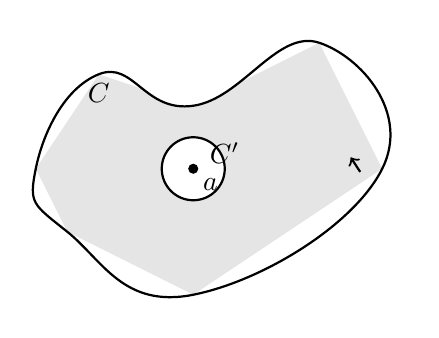
\begin{tikzpicture}[scale=0.8]
  % Fill the region between the outer loop and inner circle
  \begin{scope}
    \clip plot[smooth cycle,tension=0.8] coordinates {
      (3,0) (2,2) (0,1) (-1.5,1.5) (-2.5,0) (-2,-1) (0,-2)
    };
    \fill[gray!20] (3,0) -- (2,2) -- (0,1) -- (-1.5,1.5) -- (-2.5,0) -- (-2,-1) -- (0,-2) -- cycle;
    \fill[white] (0,0) circle (0.5);
  \end{scope}

  % Draw the outer loop
  \draw[thick] plot[smooth cycle,tension=0.8] coordinates {
    (3,0) (2,2) (0,1) (-1.5,1.5) (-2.5,0) (-2,-1) (0,-2)
  };

  % Arrow indicator on the outer loop
  \draw[->,thick] (2.65,-0.05) -- (2.5,0.18);

  % Draw the inner circle
  \draw[thick] (0,0) circle (0.5);

  % Point a at center
  \filldraw (0,0) circle (2pt) node[below right] {$a$};

  % Labels
  \node at (0.5,0.25) {$C'$};
  \node at (-1.5,1.2) {$C$};
\end{tikzpicture}
\end{center}

  灰色环域的正向边界为 \(C-C'\)，故
  \[
  \oint_C\frac{\dd z}{z-a}
  =\oint_{C'}\frac{\dd z}{z-a}
  =\int_0^{2\pi}\ii\,\dd\theta
  =2\pi\ii.
  \]
\end{enumerate}

综上，
\[
\oint_C(z-a)^n\dd z=
\begin{cases}
2\pi\ii, & n=-1\text{ 且 }a\text{ 在 }C\text{ 内部},\\
0, & \text{其他情形}.
\end{cases}
\]
若 \(C\) 不一定是正向，更一般的结果为
\[
\oint_C\frac{\dd z}{z-a}=2\pi\ii\,\operatorname{Ind}(C,a).
\]
\end{solution}
\end{question}
